\section{Interprocedural Profiling}

The first contribution we present in this thesis is an {\em interprocedural} technique for identifying the calling context that are most frequently encountered across function invocations at run-time. We show that the traditional approach for constructing a {\em Calling Context Tree} (CCT) might not be sustainable for real-world applications, as their CCTs often consist of tens of millions of nodes, making them difficult to analyze and also hurting execution time because of poor access locality. We thus introduce a novel data structure, the {\em Hot Calling Context Tree} (HCCT), in the spectrum of representations for interprocedural control flow. The HCCT is defined as the subtree of the CCT containing only its most visited nodes, which we call {\em hot}, along with their ancestors, and can be constructed independently of the CCT using fast, space-efficient algorithms for mining frequent items in data stream.

\subsection{Motivation and Contributions}
The dynamic {\em calling context} of a routine invocation is defined as the sequence of functions that are concurrently active on the run-time stack. A calling context leads to an exact program location, as it corresponds to the sequence of un-returned calls from a program’s root function to the routine invocation it is associated with.

Context-sensitive profiling information provides valuable information for program understanding, performance analysis, and runtime optimizations. Previous works demonstrated its effectiveness for tasks such as residual testing~\cite{PavlopoulouY99,Vaswani07}, function inlining~\cite{Chang92}, statistical bug isolation~\cite{Feng03,Liblit03}, performance bug detection~\cite{Nistor13}, object allocation analysis~\cite{Nethercote07}, event logging~\cite{Zhang06}, or anomaly-based intrusion detection~\cite{Bond07}.
% this is a sync with PCCE paper
Calling-context information can also be employed in unit test generation~\cite{Villazon09}, testing of sensor network applications~\cite{Lai08}, and reverse engineering of protocol formats~\cite{Lin08}.

\begin{table}[ht]
\begin{small}
\ifauthorea{}{\centering}
\begin{tabular}{|l|r r r r|}
\hline
Application & $|$Call graph$|$ & Call sites & $|$CCT$|$ & $|$Call tree$|$\\
\hline
amarok & 13\,754 & 113\,362 & 13\,794\,470 & 991\,112\,563 \\
ark & 9\,933 & 76\,547 & 8\,171\,612 & 216\,881\,324 \\
audacity & 6\,895 & 79\,656 & 13\,131\,115 & 924\,534\,168 \\
bluefish & 5\,211 & 64\,239 & 7\,274\,132 & 248\,162\,281 \\
dolphin & 10\,744 & 84\,152 & 11\,667\,974 & 390\,134\,028 \\
firefox & 6\,756 & 145\,883 & 30\,294\,063 & 625\,133\,218 \\
gedit & 5\,063 & 57\,774 & 4\,183\,946 & 407\,906\,721 \\
ghex2 & 3\,816 & 39\,714 & 1\,868\,555 & 80\,988\,952 \\
gimp & 5\,146 & 93\,372 & 26\,107\,261 & 805\,947\,134 \\
gwenview & 11\,436 & 86\,609 & 9\,987\,922 & 494\,753\,038 \\
inkscape & 6\,454 & 89\,590 & 13\,896\,175 & 675\,915\,815 \\
oocalc & 30\,807 & 394\,913 & 48\,310\,585 & 551\,472\,065 \\
ooimpress & 16\,980 & 256\,848 & 43\,068\,214 & 730\,115\,446 \\
oowriter & 17\,012 & 253\,713 & 41\,395\,182 & 563\,763\,684 \\
pidgin & 7\,195 & 80\,028 & 10\,743\,073 & 404\,787\,763 \\
quanta & 13\,263 & 113\,850 & 27\,426\,654 & 602\,409\,403 \\
sudoku & 5\,340 & 49\,885 & 2\,794\,177 & 325\,944\,813 \\
vlc & 5\,692 & 47\,481 & 3\,295\,907 & 125\,436\,877 \\
%\hline
botan & 3\,388 & 27\,114 & 308\,550 & 26\,272\,804\,980 \\
cairo-perf-trace & 1\,408 & 3\,696 & 137\,920 & 15\,976\,619\,734 \\
crafty & 107 & 516 & 36\,434\,095 & 10\,403\,074\,070 \\
fhourstones & 18 & 32 & OOM & 39\,272\,563\,944 \\
gobmk & 1\,133 & 4\,049 & OOM & 21\,909\,088\,291 \\
ice-labyrinth & 2\,335 & 8\,050 & 2\,160\,052 & 1\,637\,076\,406 \\
mount-herring & 2\,318 & 8\,269 & 3\,733\,120 & 3\,311\,257\,932 \\
overworld & 14\,173 & 50\,394 & 3\,774\,937 & 4\,112\,679\,880 \\
scotland & 13\,932 & 51\,206 & 1\,813\,368 & 5\,982\,612\,379 \\
sjeng & 57 & 221 & OOM & 28\,370\,207\,811 \\
\hline
\end{tabular}
\vspace{4mm}
\caption{\label{tab:hcct-CCTsize} Number of nodes of call graph, call tree, calling context tree, and number of distinct call sites for different applications. OOM stands for {\em Out Of Memory} (i.e., the CCT is too large to be constructed in main memory on a 32-bit architecture). Game PlanetPenguin Racer has been run on courses {\tt mount-herring} and {\tt ice-labyrinth}; similarly, game SuperTuxKart has been run on tracks {\tt overworld} and {\tt scotland}. }
\end{small}
\end{table}
\ifauthorea{\newline}{\vspace{-6mm}}

\mynote{Add reference to related work section for the CCT}
Calling context trees (CCTs) offer a compact representation for context-sensitive information. In fact, a CCT yields a more accurate profile than a {\em call graph} (which can sometimes drive to misleading conclusions~\cite{Ponder88, Spivey04}) in a space that is typically several orders of magnitude smaller than the one required to maintain a {\em call tree}. Many techniques have also been proposed over the years to reduce the overhead for its construction.
%, by trading accuracy for performance.

However, even CCTs may be very large and difficult to analyze in several applications~\cite{Bond07,Zhuang06}; their sheer size might also hurt execution time, because of poor access locality during construction and query. As an example, we report in \mytable\ref{tab:hcct-CCTsize} numbers collected for short usage sessions of off-the-shelf Linux applications and for benchmarks from popular suites. Under the optimistic assumption that each CCT node requires 20 bytes for its representation on a 32-bit architecture\footnote{From maintaining routine ID, its call site, and a performance metric as {\tt int} fields, along with two pointers for a first-child, next-sibling representation. Previous works~\cite{Ammons97,Spivey04} use larger nodes.}, nearly 1 GB of memory is needed just to maintain OpenOffice Calc's 48-million-node CCT.

In a performance profiling scenario, we remark that only the most frequent contexts are of interest, as they represent the hot spots to which optimizations must be directed. As observed in~\cite{Zhuang06}: ``Accurately collecting information about hot edges may be more useful than accurately constructing an entire CCT that includes rarely called paths.'' \myfigure\ref{fig:hcct-skewness} shows that, for different applications, only a small fraction of contexts are hot: in conformance with the Pareto principle, nearly 90\% of routine calls take place in only 10\% of contexts. The skewness of the distribution suggests that space could be greatly reduced by keeping information about hot contexts only and discarding on the fly likely cold (i.e., having low frequency) contexts.

\ifdefined\noauthorea
\begin{figure}[hb]
\begin{center}
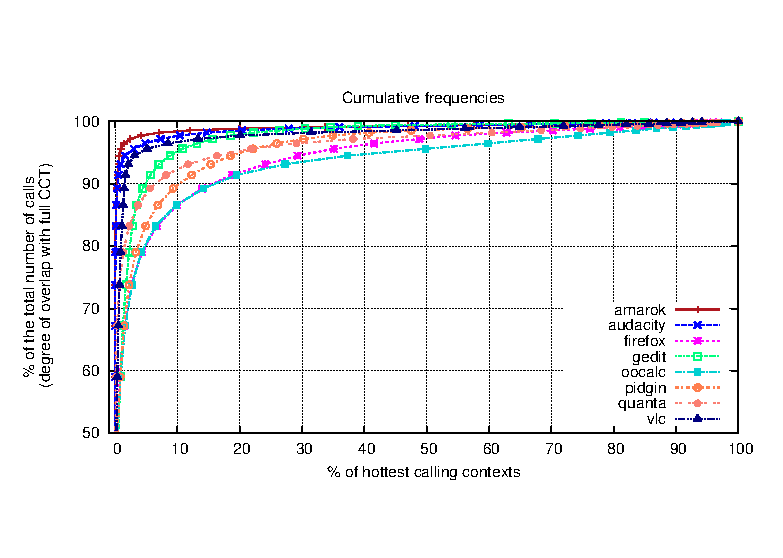
\includegraphics[width=0.95\columnwidth]{figures/hcct-skewness/hcct-skewness.eps}
\caption{\protect\label{fig:hcct-skewness} Skewness of calling contexts distribution on a representative subset of applications. For instance, in {\tt oocalc}, 10\% of the hottest calling contexts account for more than 86\% of all routine calls.
}
\end{center}
\end{figure}
\fi

\paragraph*{Contributions.} In this thesis, we introduce a novel run-time data structure, called {\em Hot Calling Context Tree (HCCT)}, that compactly represents all the hot calling contexts encountered during a program's execution, offering an additional intermediate point in the spectrum of data structures for representing interprocedural control flow. The HCCT is a subtree of the CCT that includes only hot nodes and their ancestors, also maintaining estimates of performance metrics (e.g., frequency counts) for hot calling contexts. We cast the problem of identifying the most frequent contexts into a data streaming setting: we show that the HCCT can be computed without storing the exact frequency of all calling contexts, by using fast and space-efficient algorithms for mining frequent items in data streams. These algorithms allow us to distinguish between hot and cold contexts on the fly, with the accuracy of maintained frequency estimates being formally guaranteed.

%~\cite{}

%Context-sensitive profiling provides 
%These algorithms allow us to distinguish between hot and cold context on-the-fly, and we show both theoretically and experimentally that for collected metrics the HCCT achieves a similar precision as the CCT in a space that is several orders of magnitude smaller. We show on prominent benchmarks that our implementation, shipping as a plugin for the \gcc\ compiler, incurs a slowdown competitive with the \gprof\ profiler while collecting much finer-grained profiles.

\subsection{Approach}

\paragraph*{Calling Context Trees.} A {\em calling context tree} (CCT) can be used to compactly represent all calling contexts encountered during the execution of a program. Calling contexts can be straightforwardly mapped to paths in a tree: nodes represent un-returned function calls, and each path from the root to a node $v$ encodes the calling context of the call associated with $v$. As in a tree the path from the root to any of its nodes is always unique, we can also say that each calling context is uniquely represented by a node. CCTs represent identical calling contexts just once, aggregating their metrics. A routine with multiple contexts will instead appear more than once in the tree. Slightly extended CCT definitions can also be given to bound its depth in the presence of direct recursion and to distinguish calls that take place at different call sites of the same calling procedure~\cite{Ammons97}.

%The call stack of a program can be mapped to a tree data structure by associating nodes with calls to procedures, so that each path from the root to a node $v$ represents the calling context of the call mapped to $v$. A routine with multiple contexts will appear more than once, but each calling context is represented just once in the CCT and metrics for identical contexts are aggregated.

A CCT can be constructed on-the-fly during the execution of a program. Let $v$ be a cursor pointer that points to the current context, i.e., to the node corresponding to the calling context of the currently active routine ($v$ is initialized to the CCT root node). At each routine invocation, the algorithm checks whether $v$ has a child associated with the called routine. If this is the case, the existing child is used and its metrics are updated, if necessary. Otherwise, a new child of $v$ is added to the CCT.  In both cases, the cursor is moved to the callee. Upon routine termination, the cursor is moved back to the parent node in the CCT. %This approach can be implemented either by instrumenting every routine call and return or by performing stack-walking if sampling is used to inhibit redundant profiling~\cite{AS00,W00,ZSCC06}.

\paragraph*{Introducing the HCCT.} In order to introduce the hot calling context tree, we have first to define when a context can be called hot. Let $N$ be the number of calling contexts encountered during a program's execution: $N$ equals the number of nodes of the call tree, the sum of the frequency counts of CCT nodes, as well as the number of routine invocations in the execution trace. 

\begin{definition}
A calling context is {\em hot} with respect to a frequency threshold $\phi\in[0,1]$ if and only if the frequency count of its corresponding CCT node is $\geq \lfloor\phi N\rfloor$. 
\end{definition}

\noindent Any calling context that is not hot is said to be {\em cold}. 

\begin{definition}
The {\em Hot Calling Context Tree (HCCT)} is the (unique) subtree of the CCT obtained by pruning all cold nodes that are not ancestors of a hot node.
\end{definition}

\noindent In graph theory, the HCCT corresponds to the Steiner tree of the CCT with hot nodes and the root used as terminals, i.e., to the minimal connected subtree of the CCT spanning hot nodes and the root. The HCCT includes all the hot nodes, and all its leaves are necessarily hot. An example of HCCT is given in \myfigure\ref{fig:hcct-example}(b). 

\ifdefined\noauthorea
\begin{figure}[ht]
\begin{center}
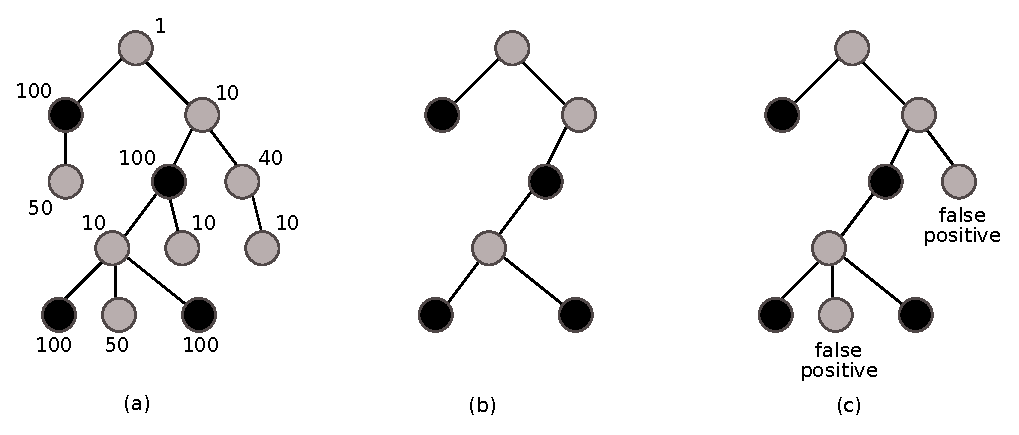
\includegraphics[width=0.95\columnwidth]{figures/hcct-example/hcct-example.eps}
\caption{\protect\label{fig:hcct-example} (a) CCT annotated with calling-context frequency counts; (b) HCCT; and (c) $(\phi,\varepsilon)$-HCCT. Hot nodes are black. In this example $N=581$, $\phi=1/10$, and $\varepsilon=1/30$: the approximate HCCT includes all contexts with frequency $\ge\lfloor\phi N\rfloor=58$  and no context with frequency $\le\lfloor(\phi-\varepsilon) N\rfloor=38$.
}
\end{center}
\end{figure}
\fi

\paragraph*{Mining Frequent Items.} Finding the space lower bound for computing the HCCT online can be reconducted to the {\em frequent items} (a.k.a. heavy hitters) problem, which has been extensively studied in data streaming computational models. Given a frequency threshold $\phi\in[0,1]$ and a stream of length $N$, the problem (in its simplest formulation) is to find all items that appear in the stream at least $\lfloor\phi N\rfloor$ times, i.e., having frequency $\ge\lfloor\phi N\rfloor$. For instance, for $\phi=0.1$ the problem seeks all items that appear in the stream at least $10\%$ of the times. Notice that at most $1/\phi$ items can have frequency larger than $\lfloor\phi N\rfloor$.  It can be proved that any algorithm that outputs an exact solution requires $\Omega(N)$ bits, even using randomization~\cite{Muthukrishnan05}. Hence, researchers focused on solving an approximate version of the problem:

\begin{definition} 
{\mbox{$(\phi,\varepsilon)$-heavy hitters problem.}} Given two parameters $\phi,\varepsilon\in[0,1]$, with $\varepsilon<\phi$, an algorithm has to return all items with frequency $\ge\lfloor\phi N\rfloor$ and no item with frequency $\le\lfloor(\phi-\varepsilon) N\rfloor$.
\end{definition} 

\noindent In the approximate solution, false negatives are not allowed, i.e., all frequent items must be returned. Instead, some false positives can exist, but their actual frequency is guaranteed to be at most $\varepsilon N$-far from the threshold $\lfloor\phi N\rfloor$. For the HCCT construction, we focus on a variant of the problem where, besides returning the heavy hitters, it is necessary to estimate accurately their true frequencies, the stream length $N$ is not known in advance, and all items in the stream have the same weight.

\paragraph*{Data Streaming Algorithms.} In the data streaming computational model, algorithms should be able to perform near-real time analyses on massive data streams, where input data come at a very high rate and cannot be stored entirely due to their huge, possibly unbounded size~\cite{Demetrescu07,Muthukrishnan05}. This line of research has been mainly motivated by networking and database applications: for instance, a relevant IP traffic analysis task consists of monitoring the packet log over a given link in order to estimate how many distinct IP addresses used that link in a given period of time. Since the stream may be very long and stream items may also be drawn from a very large universe (e.g., the set of source-destination IP address pairs), space-efficient data streaming algorithms can maintain a compact data structure that is dynamically updated upon arrival of new input data, supporting a variety of application-dependent queries. Approximate answers are allowed when it is impossible to obtain an exact solution using only limited space. Streaming algorithms are therefore designed to optimize space usage and update/query time while guaranteeing high solution quality. \mynote{Might move some text to Discussion paragraph?}

%For our purposes, we focus on counter-based algorithms that maintain frequency estimates for the heavy hitters from an unweighted stream of items whose length is not known in advance.

%track a subset of items from the input and monitor counts associated with them. For each new arrival, the algorithms decide whether to store the item or not, and, if so, what counts to associate with it. Update times are typically dominated by a small (constant) number of dictionary or heap operations. These algorithms, according to extensive experimental studies~\cite{CH08}, have superior performance with respect to space, running time, and accuracy compared to other classes of algorithm for $(\phi,\varepsilon)$-heavy hitters that have been proposed in the literature in the last 10 years.

%In this article we focus on counter-based algorithms that, according to extensive experimental studies~\cite{CH08}, have superior performance with respect to space, running time, and accuracy. Counter-based algorithms track a subset of items from the input and monitor counts associated with them. For each new arrival, the algorithms decide whether to store the item or not, and, if so, what counts to associate with it. Update times are typically dominated by a small (constant) number of dictionary or heap operations.

\paragraph*{Approximating the HCCT}. Streaming algorithms for mining frequent items can be used to solve a relaxed version of the HCCT construction problem. We thus compute an {\em Approximate Hot Calling Context Tree}, which we denote by {\em $(\phi,\varepsilon)$-HCCT}, where $\varepsilon<\phi$ controls the degree of approximation. The $(\phi,\varepsilon)$-HCCT contains all hot nodes (true positives), but may possibly contain some cold nodes without hot descendants (false positives). The true frequency of these false positives, however, is guaranteed to be at least $\lfloor(\phi-\varepsilon) N\rfloor$. Like the HCCT, the $(\phi,\varepsilon)$-HCCT can be thought of as a minimal subtree of the CCT spanning a set of $(\phi,\varepsilon)$-heavy hitters. Unlike the HCCT, a $(\phi,\varepsilon)$-HCCT is not uniquely defined, since the set of $(\phi,\varepsilon)$-heavy hitters is not unique: nodes with frequencies smaller than $\lfloor\phi N\rfloor$ and larger than $\lfloor(\phi-\varepsilon) N\rfloor$ may be either included in such a set or not.

\ifdefined\noauthorea
\begin{figure}[ht]
\begin{center}
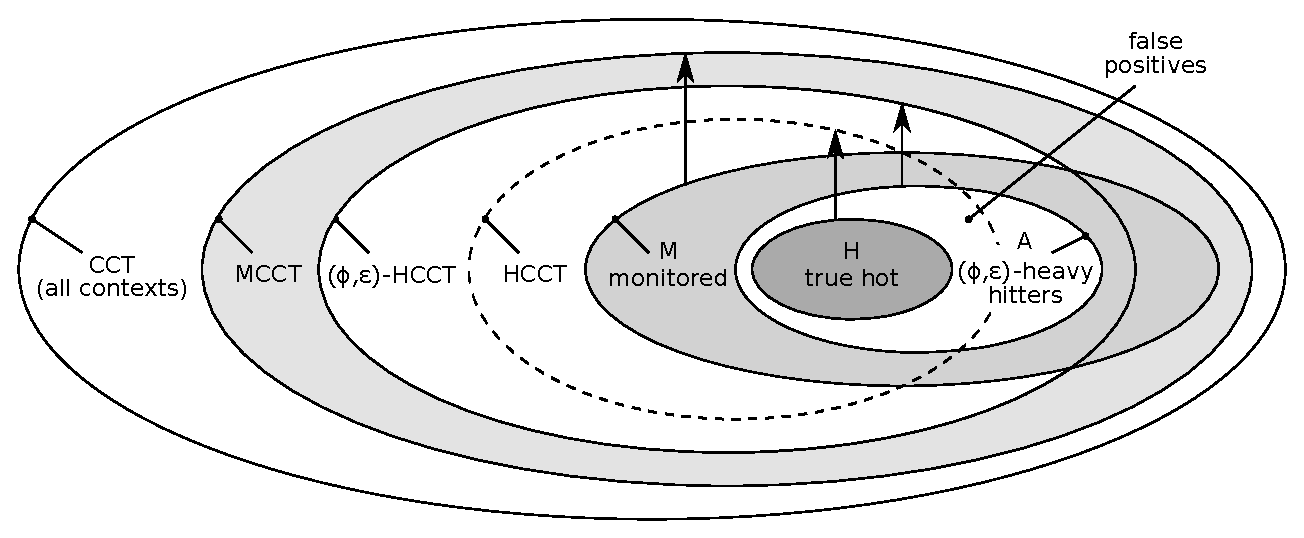
\includegraphics[width=0.95\columnwidth]{figures/hcct-venn/hcct-venn.eps}
\caption{\protect\label{fig:hcct-venn} Tree data structures and calling contexts classification. Graphical notation S $\uparrow$ T indicates that T is the minimal subtree of the CCT spanning all nodes in S.
}
\end{center}
\end{figure}
\fi 

\subsection{Algorithms}

\subsection{Implementation}

\subsection{Comparison with Related Work}

\subsection{Discussion}

% dire dello spazio asintoticamente minore